\chapter{Einleitung}

Für den Hochschulwettbewerb „Carolo-Cup“ der Technischen Universität Braunschweig soll ein autonom fahrendes Fahrzeug im Maßstab von 1:10
entwickelt werden. Im Rahmen die Arbei wird der Entwicklungsrozess der Motortreiberplatine des Fahrzeugs veranschaulicht werden.
Dabei werden auch die Probleme eines Projekts mit sich dynamisch ändernen Anforderungen gezeigt. 


\section{Carolo Cup}
Der ``Carolo-Cup'' ist ein jährlicher Hochschulwettbewerb der Technischen Universität Braunschweig dieser bietet Studenten die Möglichkeit, sich mit der Entwicklung 
und Umsetzung von autonomen Modellfahrzeugen auseinander zu setzen \cite{website-carolo-cup}. Ziel des Wettbewerbes ist es ein ein möglichst kostengünstiges
und energieeffizientes Modellfahrzeug im Maßstab 1:10 zu entwickeln. Das Fahrzeug müss dabei möglichst schnell und fehlerfrei bestimmte Aufgaben
bewältigen. Die Aufgaben werden dabei in statische und dynamische Disiplinen unterteilt. 

In den statischen Disziplinen muss das Team ihr Fahrzeugkonzept vor einer Jury, bestehend aus Experten aus Industrie und Forschung verteidigen.
Dabei wird auf die Hardware- und Softwarearchitektur sowie Energiebedarf und Herstellungskosten eingegangen. Des weiteren müssen die Lösungskonzepte
zur bewältigung der dynamischen Disziplinen vorgestellt werden.

Die dynamischen Disziplinen bestehen Dabei aus mehreren Szenarien, dem parallelen Einpaken, einem einfachen Rundkurs sowie einem Rundkurs mit Hindernissen.
Ein möglicher Rundkurs ist in Abbildung[\ref{fig:Rundkurs}] zu sehen.

\begin{figure}[H]
\centering
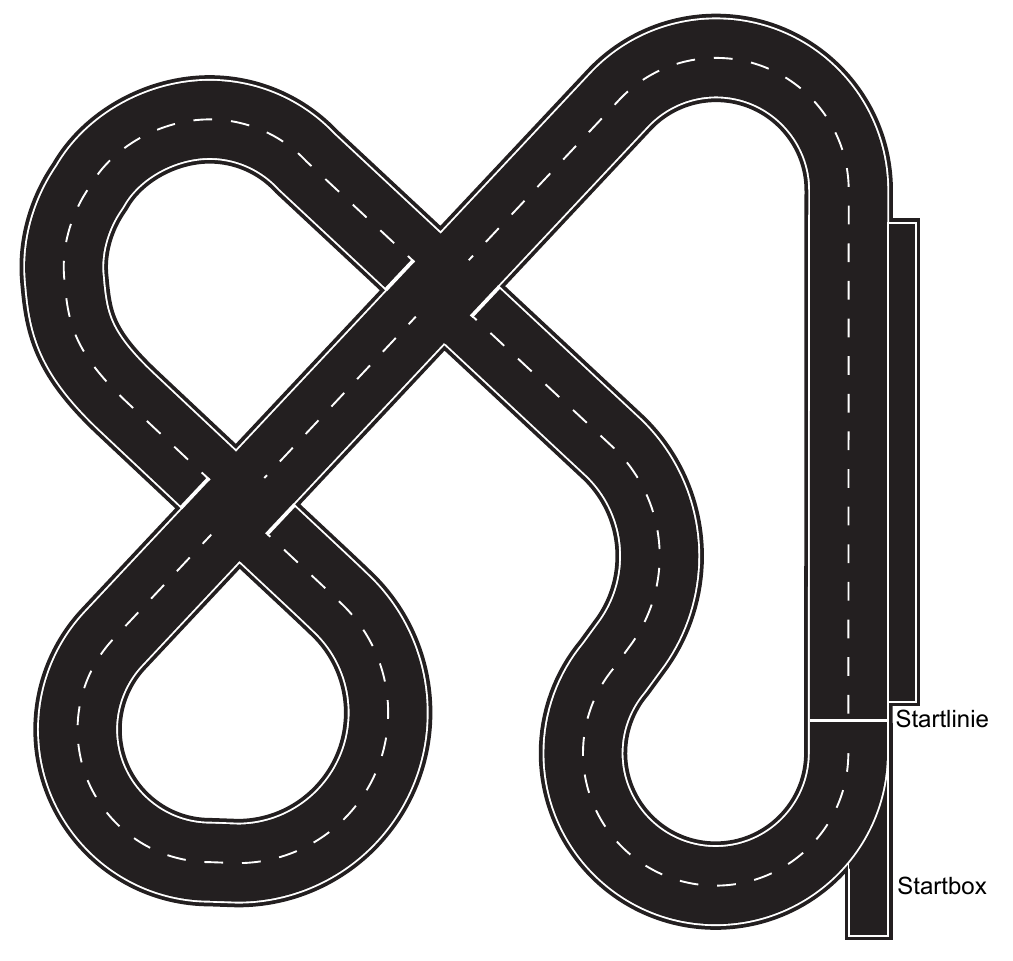
\includegraphics[width=.8\textwidth]{Strecke.png}\\
\caption{Möglicher Rundkurs \cite{website-carolo-cup-regelwerk}}
\label{fig:Rundkurs}
\end{figure}

%\section{Das Auto}

%\begin{figure}[H]
%\centering
%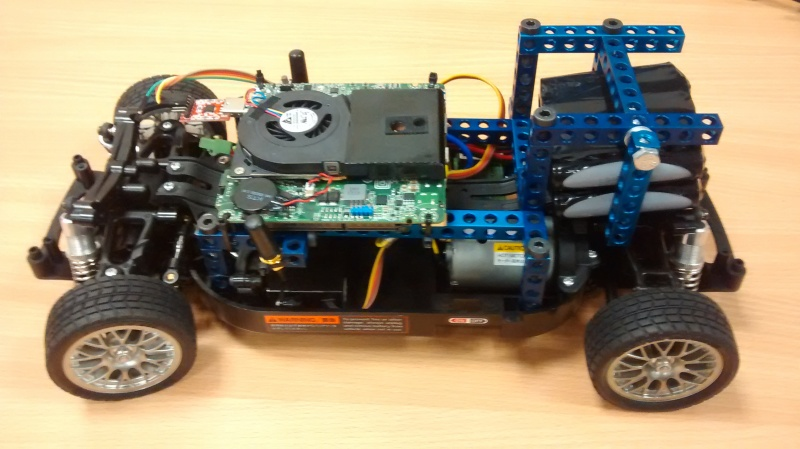
\includegraphics[width=.8\textwidth]{Auto.jpeg}\\
%\caption{Möglicher Rundkurs \cite{website-carolo-cup-regelwerk}}
%\label{fig:Auto}
%\end{figure}


\section{Aufbau der Arbeit}

Die Arbeit gliedert sich in 5 Teile???? 
In der Anforderungsanalyse wird die Ausgangssituation der Arbeit beschrieben und
analysiert welche Funktionen benötigt werden. Im Kapitel 3, dem Konzept
wird der Aufbau der Platine beschrieben und es werden grundlegende Komponenten
festgelegt. Das Umsetzungskapitel beschreibt die Umsetzung der in der Anforderungsanalyse
geforderten Funktionen. Kapitel 5 beschäftigt sich mit der Evaluierung einiger
als wichtig erachteten Komponenten und bewertet den Stromverbrauch.
Im letzten Kapitel wird das Ergebnis der Arbeit bewertet und mögliche Verbesserungen
vorgeschlagen.



